% NOTE TO AIP TYPSETERS: TO CONVERT FROM TWO-COL TO PREPRINT, SWITCH
% COMMENTOUT COMMAND FROM A TO B IE. USE:
%
%%\documentclass[prl,twocolumn,showpacs,twocolumngrid,superbib]{revtex4}
%\documentclass[prl,twocolumn,twocolumngrid,superbib]{revtex4}
%\newcommand{\commentoutB}[1]{}
%\newcommand{\commentoutA}[1]{#1}
%
% INSTEAD OF THE FOLLOWING:
%
\newcommand{\commentoutB}[1]{#1}
\newcommand{\commentoutA}[1]{}
%\documentclass[prl,aps,preprint,showpacs,superbib]{revtex4}
\documentclass[prl,aps,preprint,superbib,12pt]{revtex4}

\usepackage{graphicx}
\usepackage{amsfonts}
\usepackage{amsmath}
\usepackage{bm}
\usepackage{alltt}
\usepackage{fancyhdr}
\newcommand{\bms}[1]{{\boldsymbol #1}}
\renewcommand{\thefootnote}{\fnsymbol{footnote}}

%\draft
%\tighten
\pagestyle{fancy}

\begin{document}

\title{On the recognition of internal coordinates in various 
chemical systems}

\author{K\'aroly N\'emeth\footnotemark[1]}
\author{Matt Challacombe}

\affiliation{Theoretical Division, Los Alamos National Laboratory, Los Alamos, NM 87545, USA}

\date{\today}

\begin{abstract}
This paper presents several considerations for the appropriate choice 
of internal coordinates in various chemical systems. The appropriate
and black box recognition of internal coordinates is of fundamental 
importance
for the extension of internal coordinate algorithms to all fields where
previously Cartesian coordinates were the preferred means of geometry 
manipulations. Such fields range from local and global geometry 
optimizations to molecular dynamics as applied to a wide variety of
chemical systems. We peresent a robust algorithm that is capable 
to quickly determine the appropriate choice of internal coordinates
in a wide range of atomic arrangements.
\end{abstract}

%\pacs{31.15.-p,31.15.Ne,02.60.Pn, 45.10.Db, 02.40.Hw} 

\maketitle

\footnotetext[1]{\tt KNemeth@LANL.Gov}

\section{Introduction}
The earliest use of curvilinear internal coordinates 
in computational chemistry
is associated with vibrational analysis \cite{EWilson55}. 
It has been recognized in vibrational analysis 
that most molecular vibrations
are fairly well localized on internal coordinates that reflect
chemical concepts, such as chemical bonds, valence angles or
dihedral torsions. In fact, vibrational coupling between
appropriately chosen internal coordinates is typically
an order of magnitude smaller than in the corresponding Cartesian
representation \cite{PPulay69,GFogarasi79,GFogarasi92,PPulay77}.
This observation holds not only for harmonic but more importantly
also for anharmonic vibrational couplings.
The recognition of this reduced vibrational coupling lead to the
development of internal coordinates based geometry optimization
\cite{PPulay69,PPulay77,GFogarasi79,HSchlegel82,HSchlegel03} which
is now the standard mean of local optimization in most quantum
chemistry software packages. Internal coordinate geometry optimization
reduces the number of optimization steps typically by a factor of 2-10
for small or medium sized molecules, as compared to Cartesian
conjugate gradient algorithms \cite{TBucko05}. Another field of
potentially great use of internal coordinates is represented
by molecular dynamics \cite{PPulay02}, where research aims on developing
efficient simulation of long time-scale dynamics of large molecules.

In order to define an appropriate internal coordinate set, first
the molecular connectivity has to be determined.
The connectivity of atoms is usually recognized on the basis of 
overlapping spheres of atomic or Van der Waals radii 
\cite{VBakken02,TBucko05,KNemeth04}. Atomic radii are often not suitable
to recognize bonding in e.g. ionic salts, since typical ionic radii
may be 2-3 times larger or smaller then atomic ones 
\cite{Slater_64v41}. The application
of Van der Waals radii usually results in a huge number of 
connectivities of which most ones are neither chemically relevant nor 
helpful for the optimization. In fact an overly large number
of internal coordinates can substantially decrease the efficiency of
an internal coordinate optimizer. On the other hand, missing internal 
coordinates can lead to inefficient or non-convergent optimizations.

Besides the case of ionic systems or random clusters of atoms,
also fragmented sytems can cause problems. Consider, for example
a system of isolated molecules that interact only by very long range
forces but the intermolecular interaction cannot be described
in terms of well defined bonds such as in covalently bound systems.
E.g. two water molecules at a larger separation and at a random 
orientation, where no clear hydrogen bonding exists but there is still
a dipole-dipole interaction.
In principle the interaction of these isolated units could be treated
in terms of Cartesian coordinates of the correspondig centers 
of masses
and the appropriate rotations around them, however use of 
relative (internal) coordinates could provide a substantial advantage
in the description of the relative motions of these units.

Another very important area where internal coordinate recognition
may become troblesome is related to Van der Waals contacts.
Consider for example two strands of polymeric teflon. Which 
Van der Waals contacts should we allow for the optimization of their
structures and which ones not? The same question raises even more
importantly in biopolymers, such as proteins, when one considers
their interchain interactions. Or, also in many important
inorganic systems, e.g. in sulphur crystal where Van der Waals 
interaction determines the size and shape of the elementary cell and
may also have a considerable influence on the structure of the
covalently bound S$_{8}$ rings.

Clearly, an important disadvantage of internal coordinates 
over Cartesian ones
is that while Cartesian coordinates are always readily and
obviously at hand,
internal ones are often somewhat arbitrarily defined and thus
can provide a large, definitions-based performance difference
in geometry optimization. 
Unfortunately,
a general algorithm that would overcome this inconvenience in the use
of internal coordinates has not yet been developed. This is probably
the reason why internal coordinates based geometry manipulation
is sometimes cosidered an art rather then science.
Indeed, the problem is that in many of the
problematic systems the boundaries of the chemical concepts are 
reached while the universality of Cartesian coordinates is always 
clearly undoubted. Thus, at one hand internal coordinates offer
great advantage in geometry manipulations on the other hand their
use seems to be much less deterministic then the one of Cartesians.
In the present paper we attempt to bridge the coordinate recognition
gap between the great performance of internal coordinates and the 
troblesomeness of their definition.

\section{Rigidity and flexibility of internal coordinate systems}
Let us suppose that a highly redundant set of primitive
internal coordinates (stretches, bends, torsions, out-of-planes
and linear bendings) is
at hand and we want to reduce this set 
by selecting out the minimally necessary subset of 
primitive internal coordinates that is sufficient for succesful
geometry optimization.
On one hand, reducing the number of primitive internal coordinates
is important because this reduces the rigidity of the internal 
coordinate system and allowes for faster optimizations.
On the other hand, an internal coordinate system that represents
overly large flexibility may also be dangerous for the optimization.
For example if a folded protein would be described only by the covalent
bonds related coordinates, topologically far but spacially close
pieces of the polymer would crash into each other during the 
optimization. Thus a reasonable balance between rigidity and
flexibility must be found for a good internal coordinate system.

The rigidity of an internal coordinate system appears when
one wants to turn arbitrary internal coordinate displacements
into a displaced Cartesian structure, for example
during the course of the iterative back-transformation 
\cite{PPulay77} in a geometry optimization step. 
We define the rigidity of the internal coordinate system, $r$, 
as the norm of the difference between the desired internal coordinate 
displacements $\Delta \phi_{d}$ 
and the realized displacements $\Delta \phi_{r}$: 
\begin{equation}
r = \| \Delta \phi_{d} - \Delta \phi_{r} \| .
\end{equation}
The fundamental reason for the appearence of non-zero
rigidity in optimization steps is 
that it is impossible to predict exact, $r=0$ curvilinear
steps by the current means of geometry optimization, unless
the step is small enough or the coordinate system has a flexibility 
similar to that of the z-matrix.

Overly large flexibility can also manifest itself through the iterative
back-transformation. For example if a protein is optimized
using only its covalent-bond skeleton, an iterative 
back-transformation can easily put
topologically far but spacially close atoms in an strongly 
overlapping position, that in turn results in huge forces.

One important technique 
that reduces the rigidity in an optimization step
is based on a projection method \cite{PPulay92} that filters out
so-called first order redundancies, while usually reduces 
the step-size.

One can also investigate the covariance matrix $R$
of the rigidity vector $\Delta r = \Delta \phi_{d} - \Delta \phi_{r}$,
\begin{equation}
R = \Delta r \Delta r^{t} ,
\end{equation}
where all vectors denote column vectors. This covariance matrix,
as summed up over several optimization steps and diagonalized 
can provide linear
combinations of internal coordinates that minimize the rigidity.
A similar idea \cite{MKarplus81,AStrachan04} 
is already widely used in the construction of 
effective normal modes, e.g. on the basis of correlated velocies
(instead of $\Delta r$-s) where velocity vectors
are provided by molecular dynamics steps. Also note that the so-called
error-matrix of the geometric DIIS algorithm \cite{PPulay84} is also a
covariance matrix and its diagonalization can provide effective
normal modes.

The theory of rigidity of internal coordinate systems has 
also been discussed recently in the context of the flexibility
analysis of protein regions \cite{AJRader02}.

Internal coordinate recognition algorithms also play an important role
in structural biology and drug-design \cite{AWSchuttelkopf04,GJKleywegt03}.

In the following we describe several important conditions 
that can assist one to select an internal coordinate set 
for stuctural manipulations of large molecules.
The main driving force of all the present investigation is to study the
ways the rigidity and the flexibility of an internal 
coordinate system can be optimized for efficient geometry optimization.

\subsection{Selection based on condition number}
The most important computational operations 
that are carried out in geometry optimization 
with internal coordinates are the coordinate transformations 
\cite{PPulay77}. The coordinate transformations involve
Wilson's $B$ matrix \cite{EWilson55}, $B$, and its pseudo-inverse, $A$.
Wilson's $B$ matrix is defined as
\begin{equation}
B_{ij} = \frac{\partial \phi_{i}}{\partial x_{j}},
\end{equation}
where $\phi_{i}$ denotes the $i$-th internal coordinate and $x_{j}$
denotes the $j$-th Cartesian coordinate of the molecule.
The matrix $G_{c}$ connects the $B$ matrix with its pseudo-inverse
$A$ via the definitions
\begin{equation}
G_{c} = B^{t} B
\end{equation}
and
\begin{equation}
A = G_{c}^{-1} B^{t} ,
\end{equation}
where $G_{c}$ is an $N_{c} \times N_{c}$ matrix, with $N_{c}$ being the
number of Cartesian coordinates, and $N_{c}=3N$, for a molecule
with $N$ atoms. $G_{c}$ has $3N-6$ nonzero eigenvalues that refer to 
the internal degrees of motion of a non-linear molecule, and
$6$ zero eigenvalues referring to molecular translations and rotations. 
Thus the
matrix, $G_{c}^{-1}$ must be computed as a generalized inverse. 
Let $\lambda_{max}$ and $\lambda_{min}$ denote the maximum and minimum
of the largest $3N-6$ eigenvalues of $G_{c}$ and 
$\lambda_{c}=\lambda_{min}/\lambda_{max}$ is the condition number
of $G_{c}$. 
$\lambda_{c}$ can always be calculated once
an internal coordinate set is given. 
The first condition (Condition \#1) that any internal coordinate set
must satisfy is that the $G_{c}$ matrix calculated over the 
internal coordinates given must have $3N-6$ nonzero eigenvalues. 
This condition refers to the requirement
that the internal coordinates must span the whole space 
of internal motions of the molecule.
Once this first condition is satisfied one can think of making
selection between the actual internal coordinates and search
for a reduced set of internal coordinates that still satisfies 
Condition \#1 with the minimal number of internal coordinates, so that
rigidity can be reduced.
Say, for an $N=100$ atoms molecule $N_{i}=294$ internal coordinates
can be selected that satisfy Condition \#1. However, these $N_{i}=294$
internal coordinates can be selected in lots of different ways,
i.e. lots of sub-sets of the originally $N_{i}>294$ elements internal
coordinate set can be chosen. To make a further selection
among these subsets, Condition \#2 can be introduced:
let us choose the one among equal-sized subsets which provides the
largest $\lambda_{c}$ condition number. This way both
the size and the choice of internal coordinates can be chosen
uniquely, unless degenerate subsets occure in the $\lambda_{c}$ sense.

It is needless to say that the calculation of $\lambda_{c}$
for all possible selections of internal coordinates would be 
very demanding computationally, even if it can be done very efficiently
for each individual coordinate set using sparse matrix techniques.
Thus we consider the $\lambda_{c}$-based
selection procedure impractical for large molecules, even though it
provides a mathematically strict formulation for reducing the rigidity
of a coordinate system.

\subsection{Linear combination of primitive internal coordinates}
The condition number $\lambda_{c}$ of a given internal coordinate set
can also be modified by the construction of appropriate linear 
combinations of primarily given internal coordinates. Usually, the
primary internal coordinate set consists of so-called primitive
internal coordinates, i.e. stretchings, bendings, torsions,
out-of-planes and linear bendings. One well established set of such
linear-combinations is the so-called natural internal coordinates
\cite{GFogarasi92,MvonArnim99}. Unfortunately, the construction
of natural internal coordinates is difficult to 
automatize especially for systems that contain
lots of fused rings \cite{BPaizs00}. 

Alternatively, one can use the so-called delocalized
internal coordinates \cite{JBaker96}. Delocalized internal coordinates
provide a $3N-6$ dimensional set of linear-combined primitive
internal coordinates, where the linear combination coefficients
come from a unitary matrix, $U$. $U$ is constructed either by
diagonalizing the matrix $G_{i}=BB^{t}$ and taking eigenvectors of 
its non-zero subspace or by QR-decomposition of
$B$. Note that these two procedures result in different $U$ unitary 
matrices. The purpose of constracting $U$ is solely to use
the non-zero subspace of $G_{i}$ to get $3N-6$ linear combinations
of primitive internal coordinates. Any rotationally transformed
$U$ can be considered a legitimate linear combination as it still spans
the non-zero subspace of $G_{i}$. In practice 
only the $U$ matrices constructed by diagonalization 
\cite{JBaker96,JAndzelm92} or 
by QR-decomposition (e.g. in Ref. \onlinecite{TBucko05})
are used. The effect of the additional unitary trasnformation 
of $U$ has not been studied yet. Also note that the generation of
the delocalized internal coordinates for very large molecules 
can not be carried out in a robust fashion,
as both diagonalization and QR-decomposition are
inefficient for this purpose. While diagonalization scales cubically
with system size, sparse QR-decomposition can best achieve 
quadratic scaling.

We do not discuss further the applicability of delocalized internal 
coordinates for very large systems since our primary goal here is 
to focus on how to select primitive internals for a given molecule.

\subsection{Selection based on Cholesky factorization}
Paizs {\it et.al.} describe a technique that is based
on Cholesky factorization, to determine the $3N-6$ most independent
coordinates of a redundant internal coordinate set \cite{BPaizs00}.
The technique can be viewed as a sparse Cholesky factorization
with column pivoting (see e.g. Ref. \onlinecite{GGolub96}). 
Such a technique
is tipically used to determine trapezoidal (incomplete) Cholesky
factors of positiv semidefinite matrices, such as the $G_{i}$ matrix
in the above discussions. The idea is based on the use of
pivoting when factorizing the $G_{i}$ matrix. The most independent
$3N-6$ internal coordinates are supposed to have large pivots, 
which makes it possible to select a unique $3N-6$ dimensional
set of coordinates, unless substantial degeneracies occur.

As is well known, the application of pivoting
is a major computational bottleneck when applied in large sparse 
Cholesky factorization \cite{AGeorge81} 
since it results in a huge amount of work
in reorganizing matrices in the memory. For this reason pivoting is 
most often avoided in sparse Cholesky factorizations. Instead,
efficient symmetric permutations are used, such as the
reverse Cuthill-McKee ordering \cite{AGeorge81}, to reduce filling
of the Cholesky factors. Due to the technical difficulties,
pivoting-based coordinate selection does not seem efficient for large 
molecules.

\subsection{The von Armin approach}
I our opinion the best algorithm for practical 
coordinate recognition so far described
in the literature is the one by von Arnim and Ahlrichs 
\cite{MvonArnim99}. Here we only focus on their algorithm of 
recognizing the molecular connectivity. In this approach
atomic radii are gradually increased while overlapping atomic 
spheres are checked until the whole molecule becomes interconnected.   
In the first phase somewhat scaled atomic radii are are used
to recognize the strongest bonds. In the second phase, when 
atomic radii are increased, first hydrogen bonds are checked and 
if fragments are still not connected, bonds between any other atoms
are also allowed. 

The great advantage of the von Armin approach of
connectivity recognition against all previously
mentioned analysis is that it can be carried out in an extremely robust
fashion and does not require much use of large linear algebraic
manipulations, as opposed to e.g. pivoting-based Cholesky 
factorization or $\lambda_{c}$ based coordinate selection methods.

\section{Length-scale scanning}
\label{twoloops}
Our algorithm for the recognition of connectivity is similar
to the one of von Arnim in the sense that it also gradually scannes 
ranges of atomic radii and checks the connectivity, until all fragments
are connected. Although we carry out the same kind of length-scale
scanning, the way we do it is efficiently adapted for use in very large
molecules. Also, the intermediate steps of connectivity recognition
differ from the ones used by von Arnim.  

Our algorithm consists of two loops: loop \#1 and loop \#2.

The goal of loop \#1 is to find the shortest bonds
that build a molecular topology in which the molecule is not 
fragmented. These bonds provide a molecular skeleton, which together
with the corresponding angles (bendings, torsions, out-of-planes and 
linear-bendings) is sufficient to satisfy Condition \#1, i.e.
these coordinates span the whole space of internal motions. 

The goal of loop \#2 is to recognize those bonds, which 
have not been recognized in the first loop, because they have not been
dominant bonds in their local environment, but still have relevance
for the optimization. These bonds are usually the weaker bonds,
such as hydrogen-bonds, Van der Waals contacts or ionic
contacts.

In both loops the molecule is divided into cubes and
serial numbers of atoms falling in cubes are sorted in a sparse matrix
fashion, so that atoms of a specific cube can be identified easily. 
The linear size of the cubes starts at 3.0 \AA
and will be multiplied by a factor of 1.05 in each new cycle of the 
loops
with the purpuse of allowing longer bonds to appear within cubes and 
between neighboring cubes.
Then all possible atomic connectivities are checked within each cube 
and its neighbors in both loop \#1 and loop \#2. Thus all short-range
connectivities can be looked up efficiently.

\subsection{Loop \#1}
Before loop \#1 starts all atomic connectivities are checked for 
overlapping spheres of atoms with a radius of 1.3 times the atomic
Slater radii \cite{Slater_64v41}. 
A bond-list is formed and a sparse topology matrix is set up.
The reverse Cuthill-McKee ordering \cite{AGeorge81} is applied
to the sparse topology matrix to bring it
into a block-structured form. In this ordering unconnected 
fragments of the molecule appear as isolated blocks in the 
topology matrix. Based on this block structure, atoms are associated
with serial numbers of fragments they are part of.

Then loop \#1 starts.
In this loop atoms will be assiciated with a uniform radius
in order to find closest contacts between fragments.
This uniform radius starts at 0.75 a.u. and 
increases by a factor of 1.05 in each new cycle.
In each cycle overlap will be checked between atoms that
either belong to different fragments or are at a shorter distance
than 1.33 times a typical bondlength already attached to the
atoms of the pair being investigated. This typical bondlength
is the maximum of the shortest bondlengths of each of the atoms 
in the pair.
This latter criterion is important to avoid the formation of 
z-matrix like internal coordinate sets in several crystals, e.g.
in distorted NaCl.

Based on the updated bond-list the fragmentation of the system
is determined again and if no fragmentation occures loop \#1
terminates, otherwise repeats the above.

For most chemical systems ranging from ionic crystals through
small and medium sized organic compounds to hydrogen- 
or Van der Waals bonded crystals, loop \#1 is enough 
to determine an efficient bonding scheme for geometry optimization.  

\subsection{Loop \#2}
For some chemical systems, in which 
weak bonds connect topologically far, but spacially close units
another loop is necessary since these connectivities can 
be discovered neither on the basis of fragmentation nor by comparison
to covalent bondlengths.
For example in a folded protein the first loop may recognize only
the covalent skeleton. All weak interchain bonds must be added
afterwards. 

In loop \#2 topologically far but spacially
close units of the molecule will be connected.    
The definition of ``topologically far'' is somewhat
ambiguous. In our current recognition scheme ``topologically far''
means at least the 7th topological neighbor. This means that
smaller than 7 membered rings are not allowed to 
be closed by Van der Waals
or ionic contacts in loop \#2. We make an exception from 
this topology-based rule for 
``strong hydrogen bonds''. Our criterion for ``strong
hydrogen bond'' is that in the bond X-H$\cdot\cdot\cdot$Y
atoms X and Y must be of the atoms N,O,F,Cl and the XHY bond angle
must be smaller than 60 degrees and the X-Y distance smaller than 
3.5 \AA.

At the beginning of each cycle of loop \#2
an additional topology matrix, $T_{excl}$ is built:
\begin{equation}
T_{excl} = {(I+T_{12})}^{n_{excl}} ,
\end{equation}
where $I$ denotes the $3N \times 3N$ identity, $T_{12}$ is the 
topology matrix based on all bonds from loop \#1 and previous 
cycles of loop \#2, and $n_{excl}$ refers to ``topologically far'',
which is actually $n_{excl}=6$.
Only the symbolic part of these sparse matrices is stored 
in ordered sparse row-wise representation \cite{SPissanetzky84},
and only symbolic multiplications are carried out.
All atomic contacts will be excluded from the bond-list
that coincide with any element of the matrix $T_{excl}$. 

Loop \#2 starts with the same cube-size as loop \#1, 
and atomic radii start at 0.5 times the tabulated values of 
Van der Waals radii \cite{webelements} and are increased by a 
factor of 1.05 in each cycle while the cube size is increased
by the same factor.

This two-loops-based recognition algorithm is now the default
in our geometry optimization code and it is capable to reproduce
our previously published results on Baker's test set and enzyme 
fragments optimizations \cite{KNemeth04} while it can
be used with great efficiency in several challenging cases
enumerated later in this paper.

\section{Connectivity recognition on the basis of shell-structures}
\label{shell}
In order to simplify the above connectivity recognition, we have
tested another algorithm that is based on the investigation
of shell-structures around atoms.

For each atom $i$ an array of local bond-vectors $v_{j}$ is set up,
and stored in the matrix $L^{i}$:
\begin{equation}
L^{i}_{j} = v_{j} ,
\end{equation}
with 
\begin{equation}
v_{j}=w_{ij}*(r_{j}-r_{i})/\|r_{j}-r_{i}\| ,
\end{equation}
where $r_{i}$ and $r_{j}$ are the location vectors of the atoms $i$ and 
$j$ and $w_{ij}$ is a weight constructed by the overlap of two
hypothetical spherical Gaussian fuctions with exponents
$\xi_{i}=1/R_{i}^{2}$ and $\xi_{i}=1/R_{j}^{2}$, where
$R_{i}$ and $R_{j}$ are the corresponding atomic radii:
\begin{equation}
w_{ij}=\sqrt{(\pi/(\xi_{i}+\xi_{j}))^{3}}   
\exp{\left( -\frac{\xi_{i}\xi_{j}\|r_{j}-r_{i}\|^{2}}{\xi_{i}+\xi_{j}}\right) } .
\end{equation}
The Gaussian weights refer to a simple model of atomic orbital overlap.
For close atoms this overlap is big, for farther atoms it is small, thus
the wighting serves as a selection criteria for the importance of bonds.

The eigenvectors $U$ of the matrix $S^{i}$
\begin{equation}
S^{i} = {L^{i}}^{t} L^{i}
\end{equation}
provide principal bonding directions around atom $i$.
These principal bonding directions can be expressed in terms of
the bond vectors $v_{j}$ via the matrix $K^{i}$:
\begin{equation}
K^{i} = L^{i} U D^{-1/2} ,
\end{equation}
where $D^{-1/2}$ is a diagonal matrix and contains the generalized
inverse square-roots of the eigenvalues of $S^{i}$. Singularities
of $S^{i}$ are treated by the constraint that all eigenvalues
smaller then $0.01$ times the largest eigenvalue 
of $S^{i}$ are set to zero and are not inverted.
The total weight $W_{ij}$ of bond $ij$ among the bonds of $i$
is calculated as 
\begin{equation}
W_{ij} = \sum_{l=1}^{3} {K^{i}_{jl}}^{2} .  
\end{equation}
What remains is the filtering of bonds that are important for 
atom $i$. This is based on the assumption that unimportant
bonds will have a small enough weight. The weights $W_{ij}$ are
normalized such that they add up to one and
ordered in decreasing order. Then, the values $Q_{ij}$ are computed:
\begin{equation}
Q_{ij} = \frac{log(W_{ij})-log(W_{i(j-1)})}{log(W_{ij})-log(W_{i1})}.
\end{equation}
Note that from the above equation the index $j$ refers to decreasing
ordering in $W_{ij}$.
The values of $Q_{ij}$ refer to the statistical $Q$-test to check
whether an outlier of a series can be dropped. The tabulated Q-test
values, $Q^{t}_{j}$ for $j=[3,10]$ are: 0.94,  0.76,  0.64,  
0.56,  0.51,  0.47, 0.44, 0.41 for 90\% probability, respectively. 
If the bond-list
has only two elements, we require that the second bond should be
dropped if the first one accounts for 90\% of the total weights.
Otherwise, for a larger set of bonds, the series of allowed bonds will
terminate at that specific $k-1$-th bond, for which $Q_{ik}<Q^{t}_{k}$,
supposing that $\sum_{l=1}^{k-1} W_{il} > 0.90 $, where $0.90$
referes to 90\% of the weights. 

This simple algorithm is capable to correctly 
recognize all bonds in Baker's
test set of small and medium sized organic molecules and
reproduce our previously published geometry optimization results 
\cite{KNemeth04}. However, when some of the bonds are too long, like 
a long Van der Waals contact, this algorithm fails. More
appropriate choice of the Gaussian-based weights may though help and
the algorithm may become generally useable.

\section{Angles related internal coordinates}
\subsection{Recognition of bendings}
Our current internal coordinate generator adds all possible bond
angles (bending coordinates) to the internal coordinate list,
that is determined by nearest neighbor bonds.

\subsection{Recognition of out-of-planes}
The planarity of the vicinity of a certain atom $i$ is checked
by calculating eigenvalues of the $S$ matrix as described in Section
\ref{shell}. If the $S$ matrix has only two nonzero eigenvalues
(after the application of the constraint on the condition number of $S$)
all posible out-of-plane coordinates around atom $i$ are generated
with $i$ in the central position. Note, that we use the spectroscopic
out-of-plane coordinates \cite{EWilson55} instead of the
improper torsions of molecular mechanics.

\subsection{Recognition of torsions}
Every bond will be associated with a single torsional coordinate,
if applicable. The torsion is chosen so that the two valence angles
at the ends of the torsions should be as close to 90 degrees as 
possible, should contain the heaviest possible atoms for the terminal
positions and the terminal atoms should be those having the largest
number of topological neighbors. If fact a weight function of the form
\begin{equation}
W_{j} = \frac{(N_{j}+1)*Z_{j}}{|\pi/2-\alpha_{j}|}
\end{equation}
is used, where $j$ is a candidate atom for a terminal position of the torsion,
$N_{j}$ is the number of its nearest neighbor atoms, $Z_{j}$ is
the atomic number of $j$ and $\alpha_{j}$ is the angle $j$ closes
with the central atoms of the torsion.

\subsection{Recognition of linear bendings} 
If an angle is linear, i.e. is between 175 and 180 degrees, 
a linear bending coordinate is set up,
independent from whether the central atom has two or more neighbors.
If the terminal atoms of a linear bending have more than one
neighbors one of these neighbors will be selected to reference
the two perpendicular planes in whose intersection the linear bending is
placed. If there is no such reference, the Cartesian framework will
serve as a reference as described in Ref. \onlinecite{VBakken02}.
Note, that to each linear bending coordinate there will be
a long-range-torsion associated, that is constructed similarly to
ordinary torsions but its central atoms will be the terminal atoms
of the linear bending.
In case of collinear chains linear bendings are generated for each 
atomic triplet of the chain with an appropriate long-range torsion
that brigdes the two ends of the collinear chain.

\section{Case studies}
Here we describe three difficult cases in which finding the 
appropriate bonds turned out troublesome in earlier versions
of our default coordinate recognition algorithm.

\subsection{PETN - a high explosive with hydrogen bonds}
Pentaerythritol tetranitrate (PETN) is a high explosive 
\cite{Conant_1979}. It's crystal structure is bound together
by $C-H \cdot\cdot\cdot O-N$ type hydrogen bonds (see Pict. \ref{PETN}).
The elementary cell of PETN contains 58 atoms.
Our recognition algorithm founds 91 stretches, 174 bendings,
24 linear bendings, 101 torsions and 16 long-range torsions, 
and 36 out-of-planes. Note, that internal coordinates
that have no atom common with the central cell are not listed here.
Among the stretches, H-bond related coordinates can be divided into 
two classes: one of approximate length of $2.48$\AA, there are
16 such stretches; and the ones of length about $2.61$\AA (12 pieces).
The difficulty in recognizing the appropriate connectivity in this case
originated in the fact that if non-uniform atomic radii are used,
loop \#1 found some longer bonds for Van der Waals contacts, with 
length of about $3.14$\AA, when connected fragments that are 
isolated in the primary covalent bonding scheme.
%\commentoutA{
\begin{figure}[h]
\resizebox*{3.5in}{!}{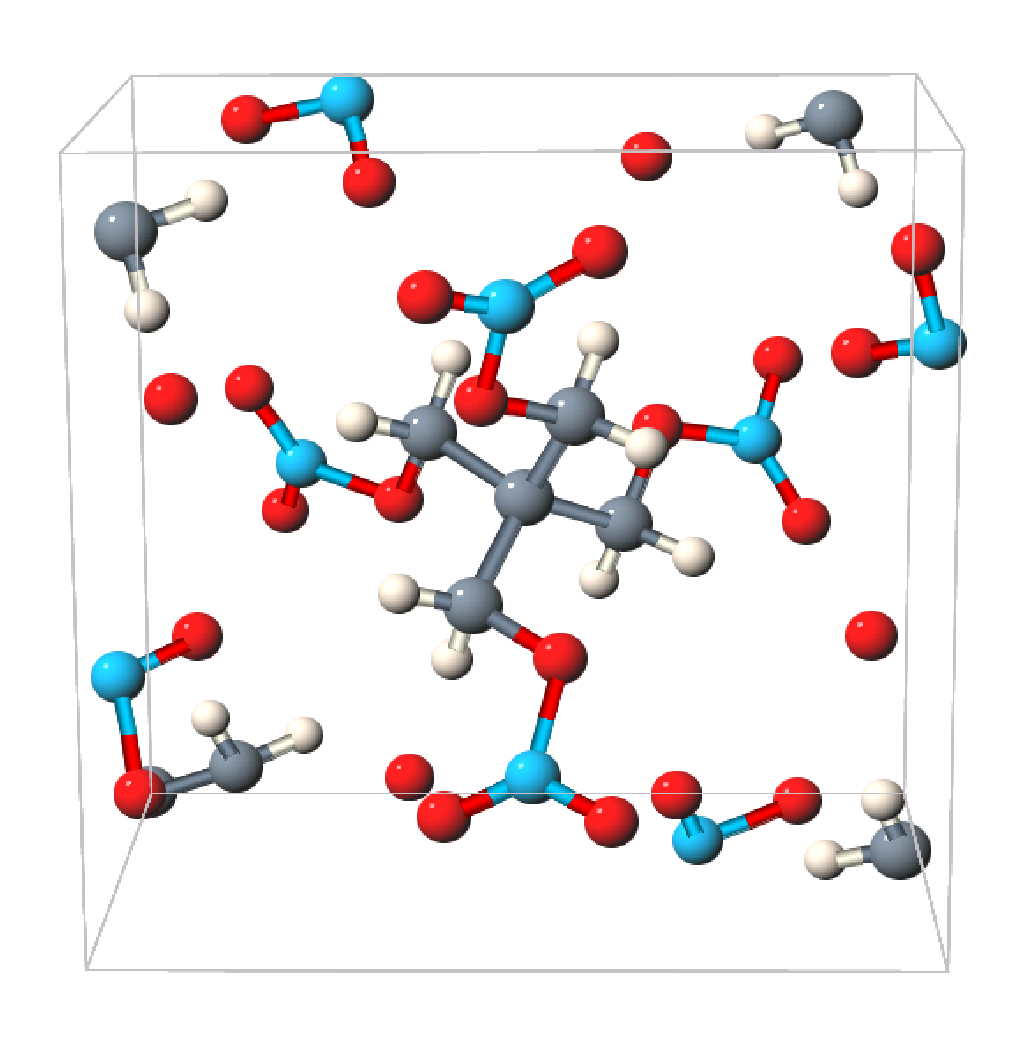
\includegraphics{PETN.eps}}
\caption{
Crystal structure of PETN.
\label{PETN}
}
\end{figure}
%}

\subsection{Teflon crystal}
The crystal of teflon (poly-tetrafluoro-ethylene) is held
together by Van der Waals contacts (see Pict. \ref{teflon}).
In our model a 156 atoms elementary cell was used.
Our recognition scheme found 244 stretches, 204 of them 
ordinary covalent bonds, and 40 Van der Waals contacts of approximate
length of $2.60-2.85$\AA. These bonds are associated with 607
bendings and 281 torsions. Note, that the number of intermolecular
bods also depends on the topological exclusion principle
presented in Section \ref{twoloops}.
%\commentoutA{
\begin{figure}[h]
\resizebox*{3.5in}{!}{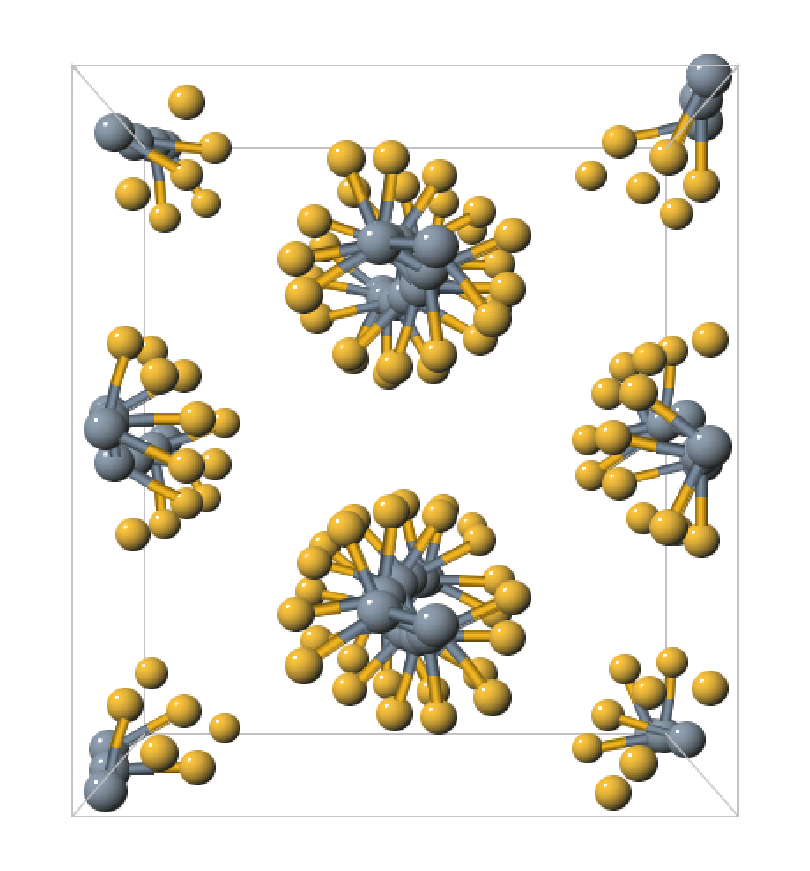
\includegraphics{teflon.eps}}
\caption{
Crystal structure of teflon.
\label{PETN}
}
\end{figure}
%}

\subsection{Distorted Sodium Chloride}
Distorted sodium chloride occured during optimization 
with a previous version of
our internal coordinates recognition scheme. 
It also modells well the case of molten ionic crystals and,
in general the case, when atomic radii are very pure approximations
to discover bonding. The elementary cell consist of two atoms.
All 27 seven stretches have been recognized that connect nearest
sodium-sodium, cloride-chloride and sodium-chloride ions.
Note, that changing the factor of $1.33$ (multiplyer for ``typical''
bond-length, see Section \ref{twoloops}) to a smaller value, say
1.2 results in the recognition of sodium-chloride interactions only.
In the default algorithm, 276 bendings, 80 linear bendings,
63 ordinary torsions and 51 long-range torsions have been detected.
Clearly, this represents a quite redundant coordinate system for 
sodium-chloride, as the stretches alone should be enough for the
optimization.

\subsection{Optimization characteristics for teflon}
In this paper we present optimization characteristics
for teflon, only. A more detailed paper about our recently 
developed crystal structure optimizer we be published separately.
Note, that for the Van der Waals contacts we have not used
the so-called ``5/R'' coordinates, as suggested elsewhere
\cite{JBaker00,TBucko05}. All optimizations have been carried out with
the QUICCA algorithm \cite{KNemeth04} as modified for crystals.
Energies and forces have been computed on the PBE/STO-3G level of
theory. Optimization was considered converged after all
atomic and lattice gradients decreased below 0.0005 a.u..
The teflon system has been optimized in 54 steps from a geometry
with initial gradients as large as 0.601103 a.u. in magnitude.
The energy curve has a smooth decline, while gradient curves 
show slow decline for the intermolecular forces. One possible 
source of improvement in this decline 
could be the application of "5/R" coordinates.
%\commentoutA{
\begin{figure}[h]
\resizebox*{3.5in}{!}{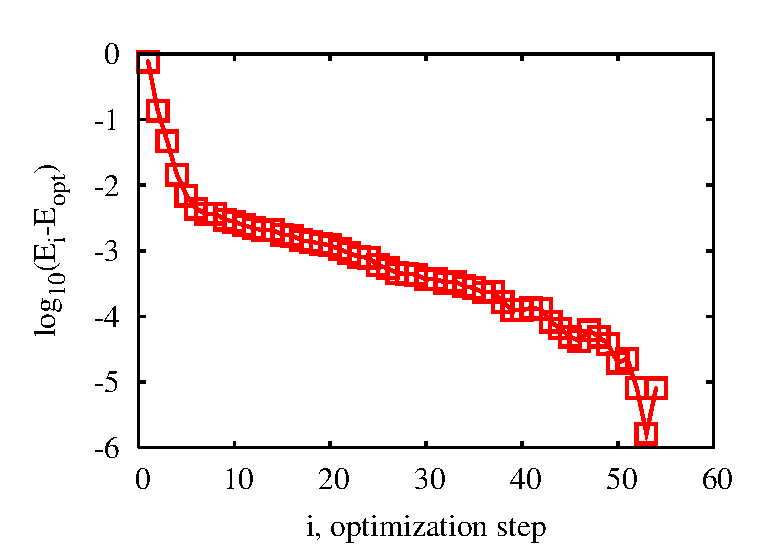
\includegraphics{energ.eps}}
\caption{
Convergence of the energy during the optimization of teflon.
\label{PETN}
}
\end{figure}
%}
%\commentoutA{
\begin{figure}[h]
\resizebox*{3.5in}{!}{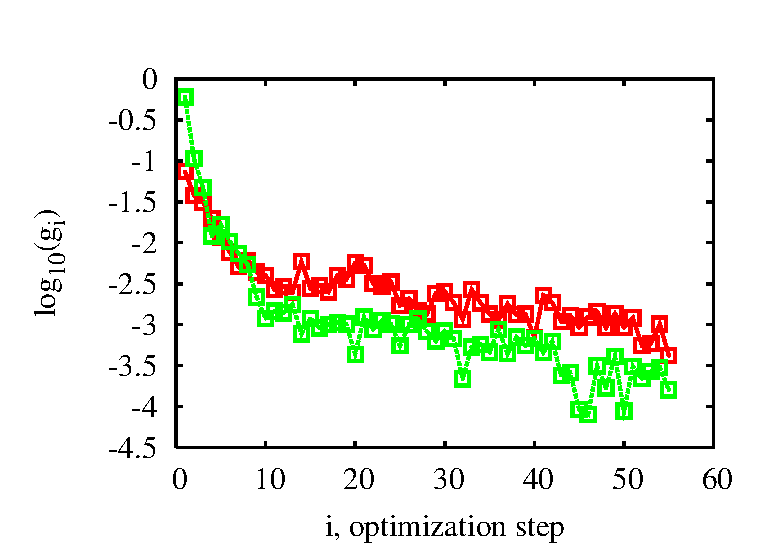
\includegraphics{grads.eps}}
\caption{
Convergence of the maximum atomic (lower curve) 
and lattice (upper curve)
forces during the optimization of teflon.
\label{PETN}
}
\end{figure}
%}

\section{Conclusions} \label{Conclusions}
We have discussed strengths and weaknesses of 
existing algorithms for the selection of 
internal coordinates for the purpose of molecular geometry optimization.
We have recommended new, robust algorithms that are capable
to recognize efficient coordinate systems for topologically
complex atomic arrangements that span the range from ionic melts to
Van der Waals bonded crystals. With the algorithms
described in the present paper we have contributed to the development 
of internal coordinate recognition that aims on generalizing the
use of internal coordinates for all situations 
where Cartesian coordinates have been the preferred mean
geometry manipulation. We have enumerated difficult cases 
in coordinate recognition and provided robust solutions that proved to
work well in complex, practical recognition tasks.

\bibliography{../../Bib/mondo_new}



\end{document}

